\begin{pr}$ $
\begin{enumerate}[(a)]
\item
\tikzstyle{b} = [rectangle, draw, fill=blue!20, node distance=6cm, text width=6em, text centered, rounded corners, minimum height=4em, thick]
\tikzstyle{g} = [rectangle, draw, fill=green!20, node distance=6cm, text width=6em, text centered, rounded corners, minimum height=4em, thick]
\tikzstyle{R} = [rectangle, draw, fill=red!20, node distance=6cm, text width=6em, text centered, rounded corners, minimum height=4em, thick]
\tikzstyle{c} = [rectangle, draw, minimum height=15em, minimum width=10em, dashed]
\tikzstyle{r} = [midway, right]
\tikzstyle{u} = [midway, above]
\tikzstyle{l} = [pos=0.25, above]

\resizebox{12cm}{3cm}{
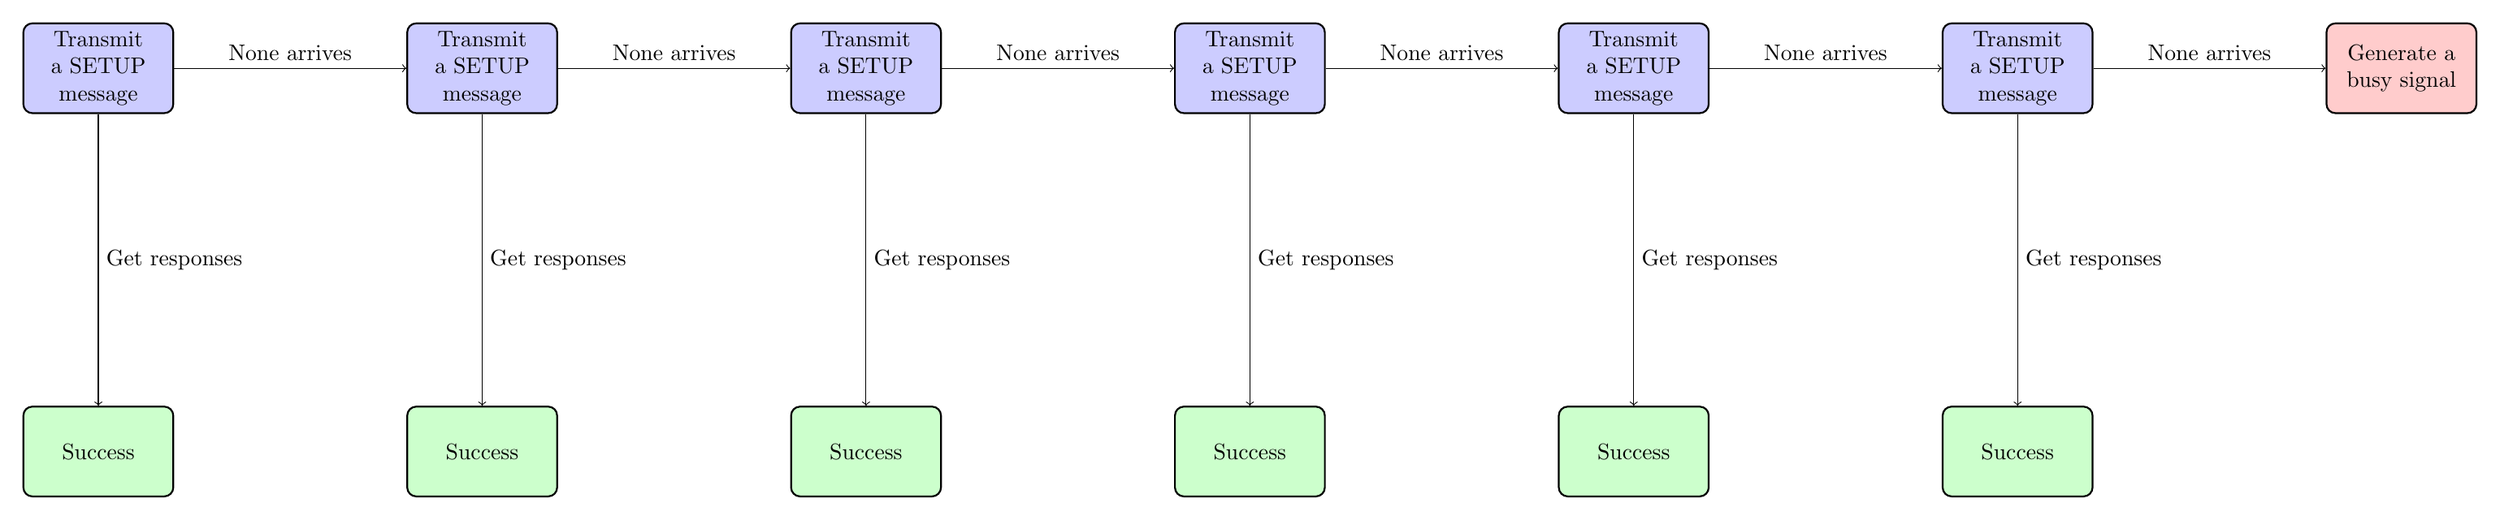
\begin{tikzpicture}[auto]
	\node [b] (a) {Transmit a SETUP message};
	\node [b, right of=a] (b) {Transmit a SETUP message};
	\node [b, right of=b] (c) {Transmit a SETUP message};
	\node [b, right of=c] (d) {Transmit a SETUP message};
	\node [b, right of=d] (e) {Transmit a SETUP message};
	\node [b, right of=e] (f) {Transmit a SETUP message};
	\node [R, right of=f] (g) {Generate a busy signal};
	\node [g, below of=a] (h) {Success};
	\node [g, below of=b] (i) {Success};
	\node [g, below of=c] (j) {Success};
	\node [g, below of=d] (k) {Success};
	\node [g, below of=e] (l) {Success};
	\node [g, below of=f] (m) {Success};

	\draw [->] (a) -- (b) node [u] {None arrives};
	\draw [->] (b) -- (c) node [u] {None arrives};
	\draw [->] (c) -- (d) node [u] {None arrives};
	\draw [->] (d) -- (e) node [u] {None arrives};
	\draw [->] (e) -- (f) node [u] {None arrives};
	\draw [->] (f) -- (g) node [u] {None arrives};
	\draw [->] (a) -- (h) node [r] {Get responses};
	\draw [->] (b) -- (i) node [r] {Get responses};
	\draw [->] (c) -- (j) node [r] {Get responses};
	\draw [->] (d) -- (k) node [r] {Get responses};
	\draw [->] (e) -- (l) node [r] {Get responses};
	\draw [->] (f) -- (m) node [r] {Get responses};

%    \node [b] (init) {Clear iptable};
%    \node [b, below of=init] (default) {Default DROP};
%    \node [b, below of=default] (icmp) {ACCEPT ICMP (no port number)};
%    \node [b, below of=icmp] (http) {ACCEPT HTTP (port: 80)};
%    \node [b, below of=http] (dns) {ACCEPT DNS (port: 53)};
%    \node [b, below of=dns] (ssh) {ACCEPT SSH (port: 22)};
%    \node [b, below of=ssh] (ftp) {ACCEPT FTP (port: 20, 21)};
%    \node [b, below of=ftp] (telnet) {ACCEPT Telnet (port: 23)};
%    \node [R, left of=telnet, node distance=6cm] (drop) {DROP};
%    \node [g, right of=dns, node distance=6cm] (accept) {ACCEPT};
%
%    \draw [->] (init) -- (default) node [r] {all};
%    \draw [->] (default) -- (icmp) node [r] {all};
%    \draw [->] (icmp) -- (http) node [r] {others};
%    \draw [->] (http) -- (dns) node [r] {others};
%    \draw [->] (dns) -- (ssh) node [r] {others};
%    \draw [->] (ssh) -- (ftp) node [r] {others};
%    \draw [->] (ftp) -- (telnet) node [r] {others};
%    \draw [->] (telnet) -- (drop) node [u] {others};    
%
%    \draw [->] (icmp) -| (accept) node [l] {ICMP};
%    \draw [->] (http) -| (accept) node [l] {HTTP};
%    \draw [->] (dns) -- (accept) node [u] {DNS};
%    \draw [->] (ssh) -| (accept) node [l] {SSH};
%    \draw [->] (ftp) -| (accept) node [l] {FTP};
%    \draw [->] (telnet) -| (accept) node [l] {Telnet};

\end{tikzpicture}
}
\item $P_K(k)=\begin{cases}
\underbrace{(1-p)^{k-1}}_{\text{The first }k-1\text{ tries fail}}\underbrace{p}_{\text{The }k\text{-th try successes}}\text{, if }1\leq k\leq5\\
\underbrace{(1-p)^5}_{\text{The first }5\text{ tries fail}}\text{, if }k=6\\
0\text{, otherwise}.
\end{cases}$.
\item It is the probability the all $6$ tries fail, which is $(1-p)^6$.
\item The probability that all $n$ tries fail $=(1-0.9)^n<0.02$.\\
$\then n=2$ is sufficient since $0.1^2=0.01<0.02$.
\end{enumerate}
\end{pr}
